\chapter{Caso Circunferencia}
\label{ch:caso_circunferencia}

En este capítulo analizamos el comportamiento de los ceros de polinomios ortogonales de Sobolev en el caso complejo, donde las medidas están soportadas en circunferencias. Este enfoque nos permite extender nuestro estudio más allá del eje real y comprender mejor los fenómenos de distribución de ceros en el plano complejo.

% CASOS SECUENCIALMENTE DOMINADOS
\textbf{Ejemplo 1.} % Originalmente Ejemplo 1
$\langle p(z),q(z) \rangle=\int_{S_{0}(1)} p(z)\overline{q(z)}\, dm_{0;1} + \int_{S_{0.4}(0.4)} p'(z)\overline{q'(z)}\, dm_{0.4;0.4}$

\begin{center}
	\begin{minipage}{0.48\textwidth}
		\centering
		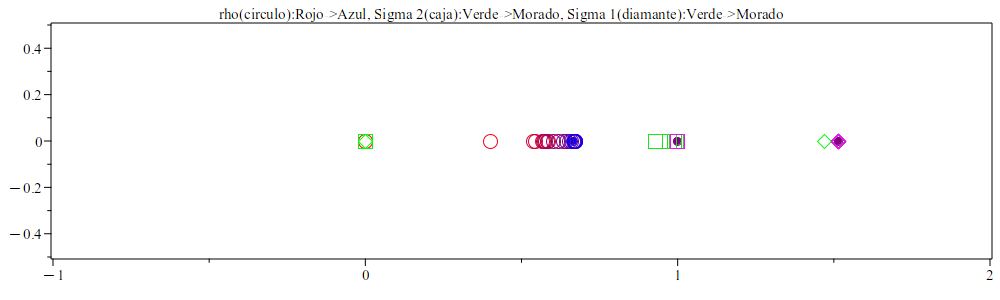
\includegraphics[width=\textwidth]{include/r1_1c1_0r2_0.4c2_0.4.png}
	\end{minipage}%
	\hfill
	\begin{minipage}{0.48\textwidth}
		\centering
		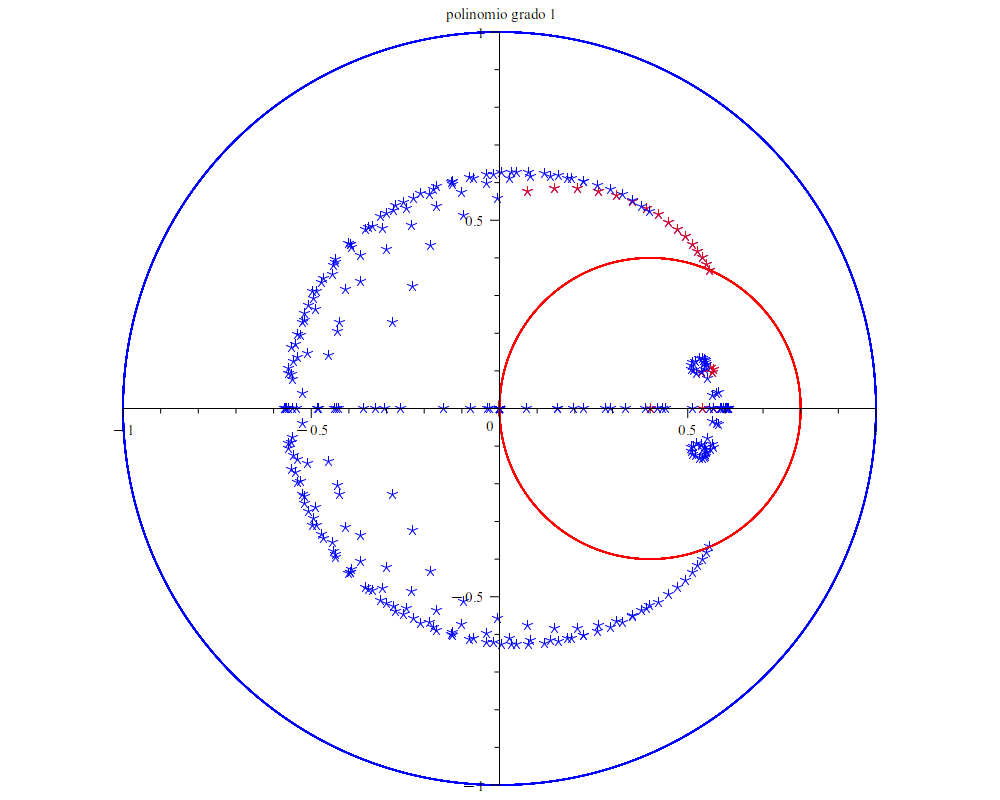
\includegraphics[width=\textwidth]{include/r1_1c1_0r2_0.4c2_0.4_zeros.png}
	\end{minipage}
\end{center}

\begin{enumerate}
	\item $\lim_{n \to 50}\sigma_{1,n}=\infty$
	\item $\lim_{n \to 50} \rho(\mathcal{D}_{n})=1.000$
	\item $\max\{Z_{n}\}_{n=0}^{50}=1.172$
	\item $\lim_{n \to 50}\sigma_{2,n}=0.998$
\end{enumerate}

\textbf{Ejemplo 2.} % Originalmente Ejemplo 3
$\langle p(z),q(z) \rangle=\int_{S_{0}(1)} p(z)\overline{q(z)}\, dm_{0;1} + \int_{S_{0.5}(10)} p'(z)\overline{q'(z)}\, dm_{0.5;10}$

\begin{center}
	\begin{minipage}{0.48\textwidth}
		\centering
		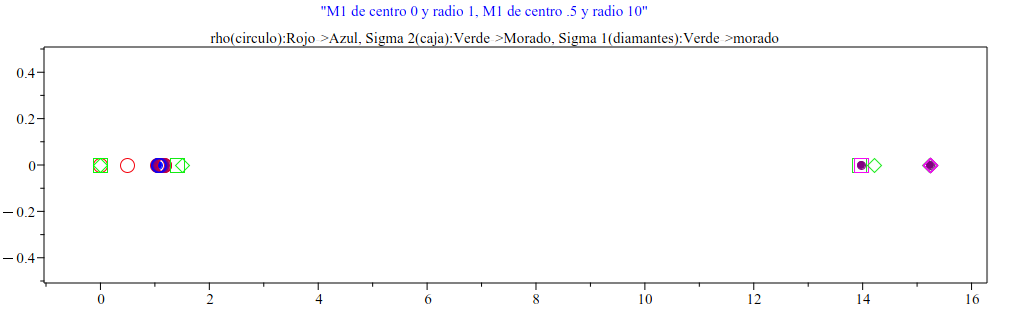
\includegraphics[width=\textwidth]{include/r1_1c1_0r2_10c2_0.5.png}
	\end{minipage}%
	\hfill
	\begin{minipage}{0.48\textwidth}
		\centering
		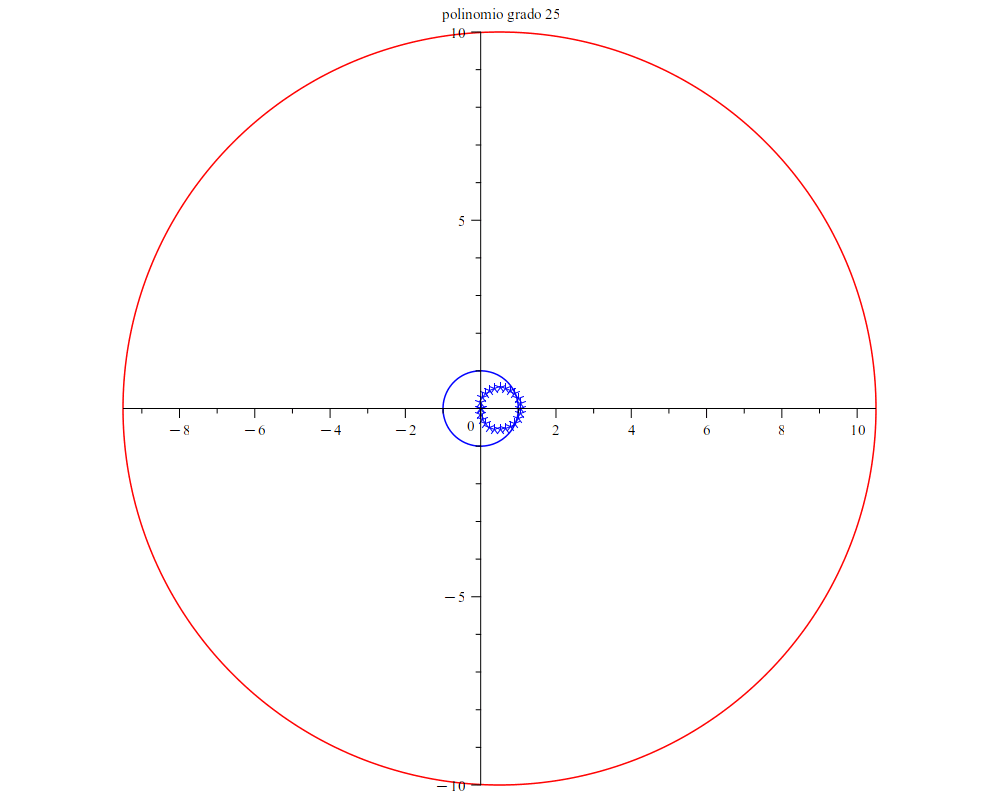
\includegraphics[width=\textwidth]{include/r1_1c1_0r2_10c2_0.5_zeros.png}
	\end{minipage}
\end{center}

\begin{enumerate}
	\item $\lim_{n \to 50}\sigma_{1,n}=\infty$
	\item $\lim_{n \to 50} \rho(\mathcal{D}_{n})=2.632$
	\item $\max\{Z_{n}\}_{n=0}^{50}=3.148$
	\item $\lim_{n \to 50}\sigma_{2,n}=1.997$
\end{enumerate}

% CASOS NO SECUENCIALMENTE DOMINADOS
\textbf{Ejemplo 3.} % Originalmente Ejemplo 2
$\langle p(z),q(z) \rangle=\int_{S_{0}(1)} p(z)\overline{q(z)}\, dm_{0;1} + \int_{S_{1}(1)} p'(z)\overline{q'(z)}\, dm_{1;1}$

\begin{center}
	\begin{minipage}{0.48\textwidth}
		\centering
		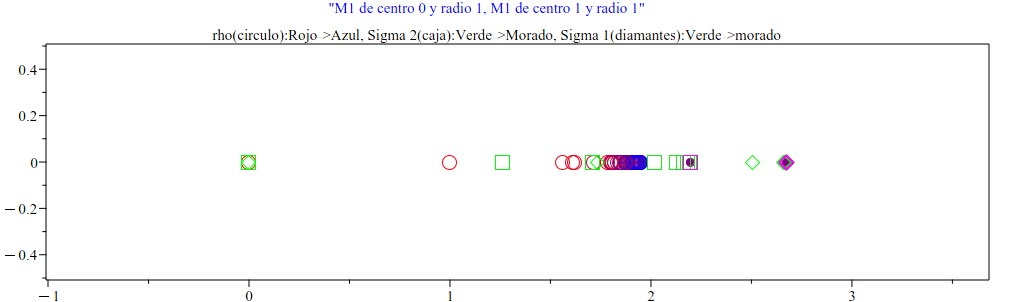
\includegraphics[width=\textwidth]{include/r1_1c1_0r2_1c2_1.png}
	\end{minipage}%
	\hfill
	\begin{minipage}{0.48\textwidth}
		\centering
		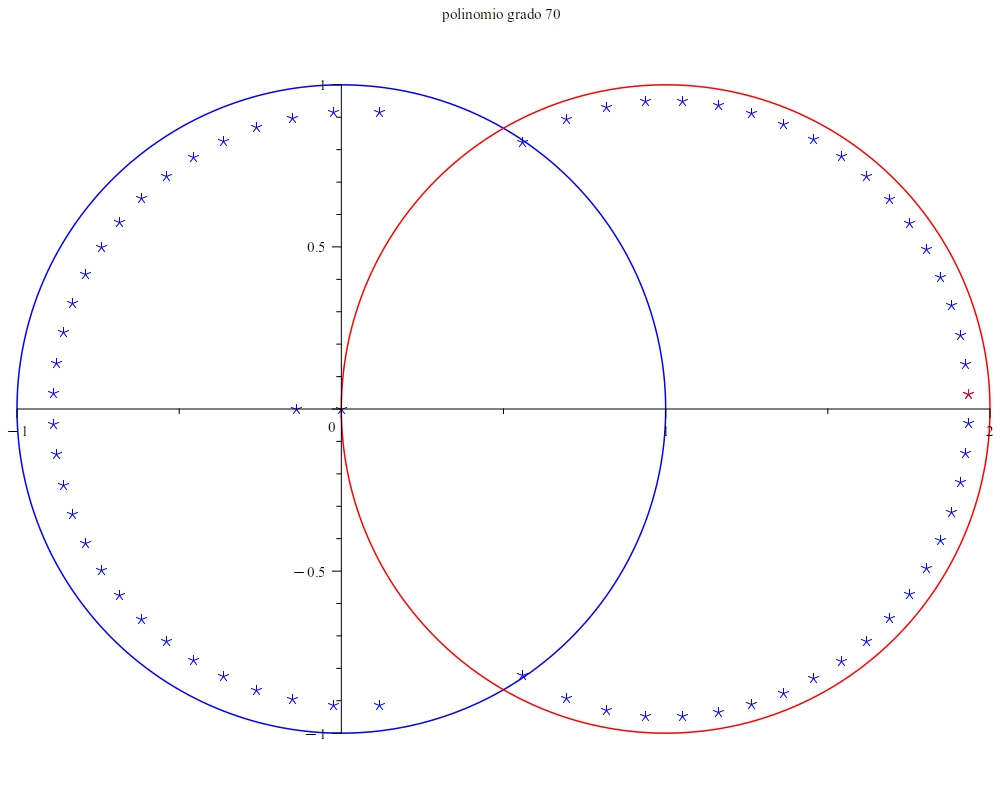
\includegraphics[width=\textwidth]{include/r1_1c1_0r2_1c2_1_zeros.png}
	\end{minipage}
\end{center}

\begin{enumerate}
	\item $\lim_{n \to 50}\sigma_{1,n}=2.192$
	\item $\lim_{n \to 50} \rho(\mathcal{D}_{n})=0.999$
	\item $\max\{Z_{n}\}_{n=0}^{50}=1.285$
	\item $\lim_{n \to 50}\sigma_{2,n}=0.998$
\end{enumerate}

\textbf{Ejemplo 4.} % Originalmente Ejemplo 4
$\langle p(z),q(z) \rangle=\int_{S_{0}(1)} p(z)\overline{q(z)}\, dm_{0;1} + \int_{S_{-10}(1)} p'(z)\overline{q'(z)}\, dm_{-10;1}$

\begin{center}
	\begin{minipage}{0.48\textwidth}
		\centering
		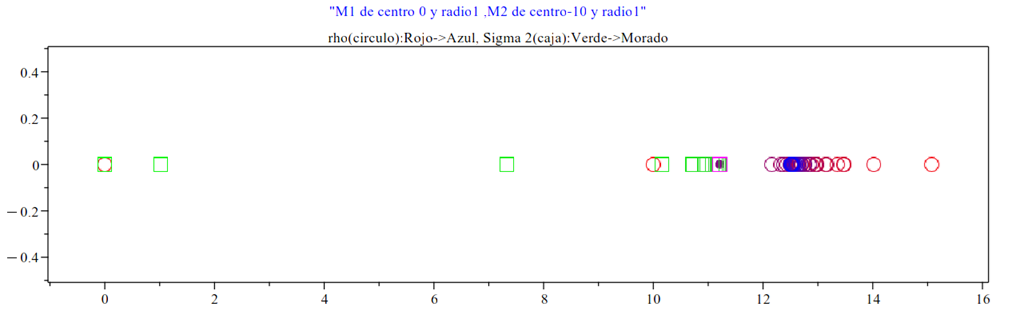
\includegraphics[width=\textwidth]{include/r1_1c1_0r2_1c2_-10.png}
	\end{minipage}%
	\hfill
	\begin{minipage}{0.48\textwidth}
		\centering
		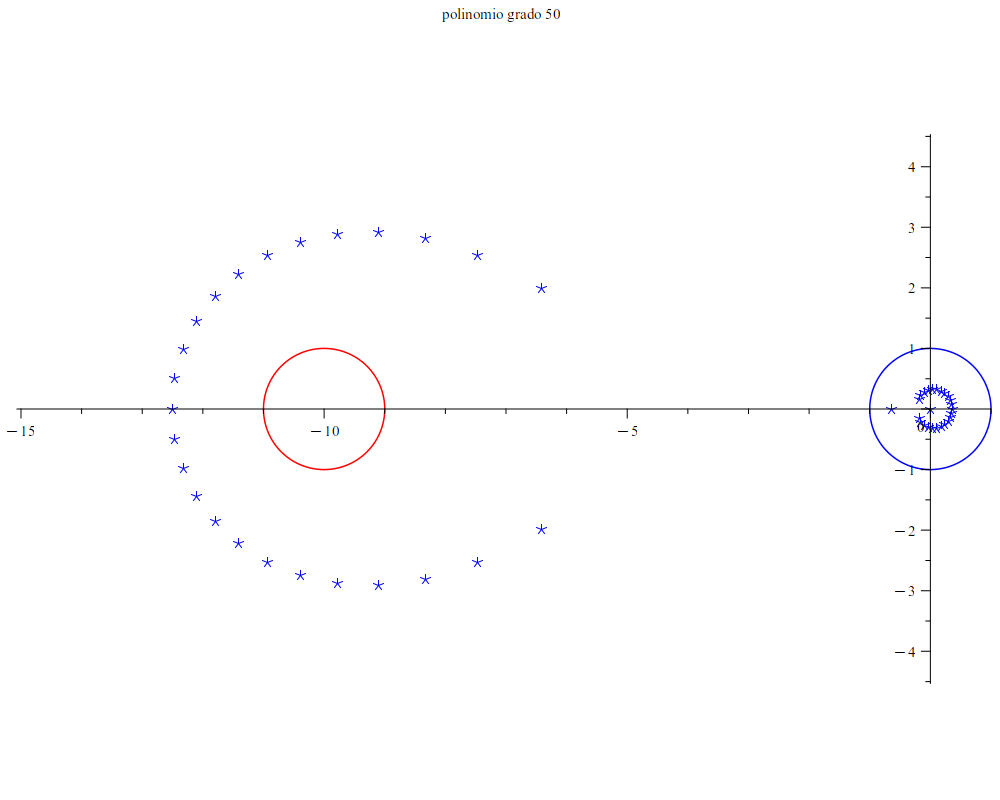
\includegraphics[width=\textwidth]{include/r1_1c1_0r2_1c2_-10_zeros.png}
	\end{minipage}
\end{center}

\begin{enumerate}
	\item $\lim_{n \to 50}\sigma_{1,n}=\infty$
	\item $\lim_{n \to 50} \rho(\mathcal{D}_{n})=2.498$
	\item $\max\{Z_{n}\}_{n=0}^{50}=2.499$
	\item $\lim_{n \to 50}\sigma_{2,n}=2.497$
\end{enumerate}

\textbf{Ejemplo 5.} % Originalmente Ejemplo 6
$\langle p(z),q(z) \rangle=\int_{S_{-10}(0.25)} p(z)\overline{q(z)}\, dm_{-10;0.25} + \int_{S_{0}(1)} p'(z)\overline{q'(z)}\, dm_{0;1}$

\begin{center}
	\begin{minipage}{0.48\textwidth}
		\centering
		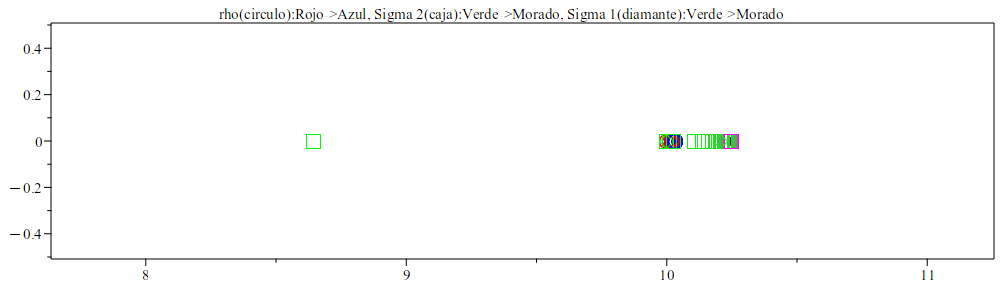
\includegraphics[width=\textwidth]{include/r1_0.25c1_-10r2_1c2_0.png}
	\end{minipage}%
	\hfill
	\begin{minipage}{0.48\textwidth}
		\centering
		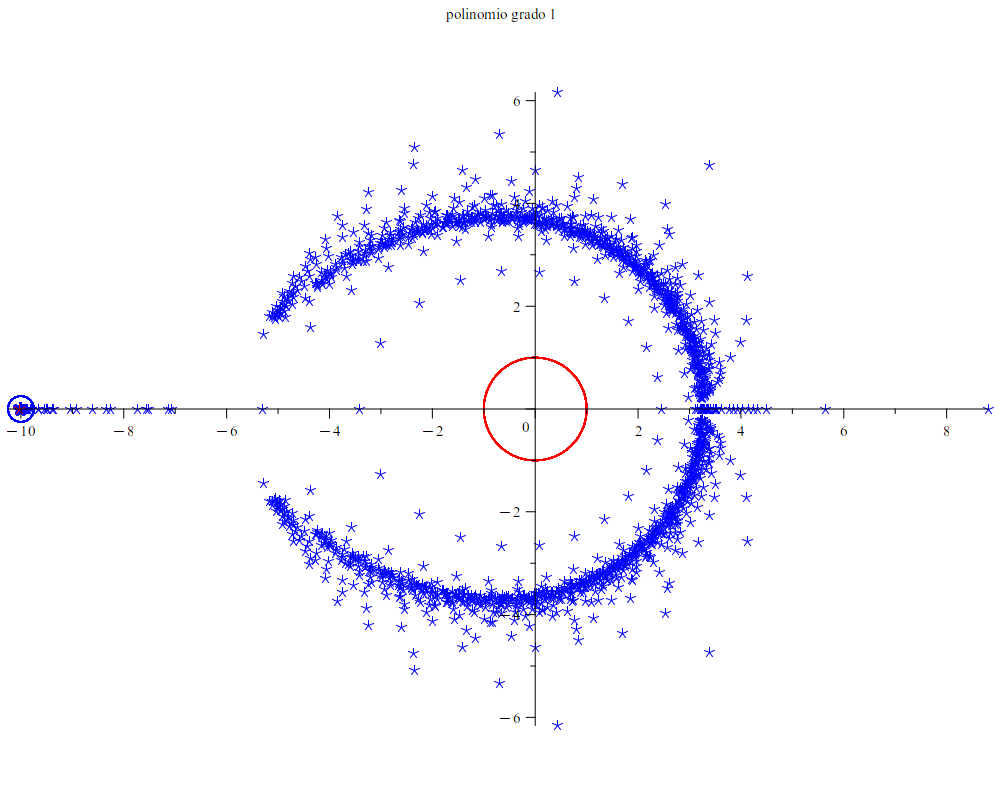
\includegraphics[width=\textwidth]{include/r1_0.25c1_-10r2_1c2_0_zeros.png}
	\end{minipage}
\end{center}

\begin{enumerate}
	\item $\lim_{n \to 50}\sigma_{1,n}=\infty$
	\item $\lim_{n \to 50} \rho(\mathcal{D}_{n})=1.998$
	\item $\max\{Z_{n}\}_{n=0}^{50}=1.999$
	\item $\lim_{n \to 50}\sigma_{2,n}=1.997$
\end{enumerate}

\textbf{Ejemplo 6.} % Nuevo ejemplo
$\langle p(z),q(z) \rangle=\int_{S_{0}(1)} p(z)\overline{q(z)}\, dm_{0;1} + \int_{S_{-10}(0.25)} p'(z)\overline{q'(z)}\, dm_{-10;0.25}$

\begin{center}
	\begin{minipage}{0.48\textwidth}
		\centering
		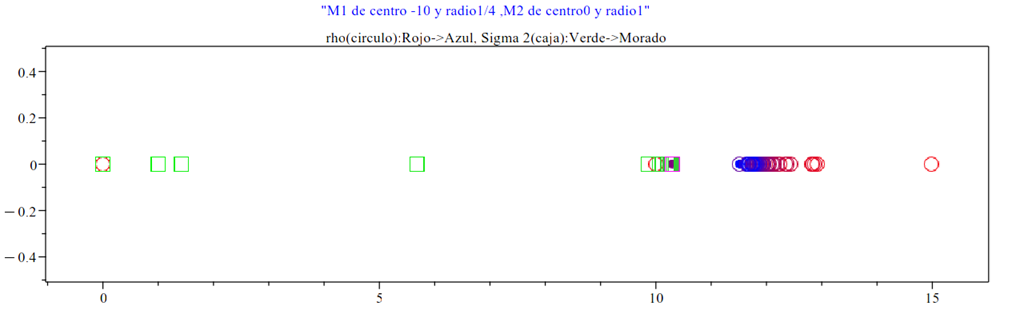
\includegraphics[width=\textwidth]{include/r1_1c1_0r2_0.25c2_-10.png}
	\end{minipage}%
	\hfill
	\begin{minipage}{0.48\textwidth}
		\centering
		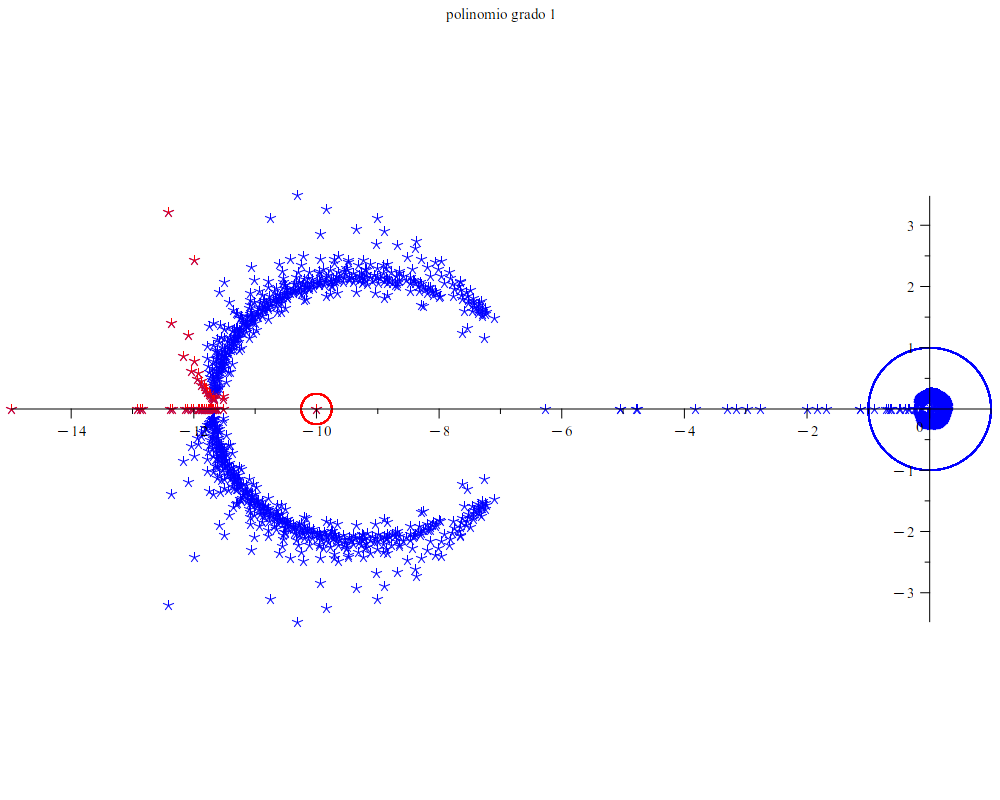
\includegraphics[width=\textwidth]{include/r1_1c1_0r2_0.25c2_-10_zeros.png}
	\end{minipage}
\end{center}

\begin{enumerate}
	\item $\lim_{n \to 50}\sigma_{1,n}=\infty$
	\item $\lim_{n \to 50} \rho(\mathcal{D}_{n})=2.498$
	\item $\max\{Z_{n}\}_{n=0}^{50}=2.499$
	\item $\lim_{n \to 50}\sigma_{2,n}=2.497$
\end{enumerate}

% CASOS CON ÁTOMO
\textbf{Ejemplo 7.} % Originalmente Ejemplo 5
$\langle p(z),q(z) \rangle=\int_{S_{0}(1)} p(z)\overline{q(z)}\, dm_{0;1} + p'(0.5+0.5i)\overline{q'(0.5+0.5i)}$

\begin{center}
	\begin{minipage}{0.48\textwidth}
		\centering
		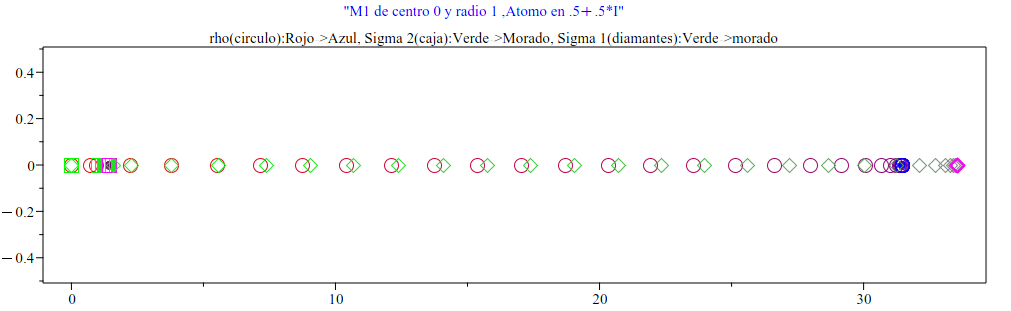
\includegraphics[width=\textwidth]{include/r1_1c1_0c2_(0.5)(0.5).png}
	\end{minipage}%
	\hfill
	\begin{minipage}{0.48\textwidth}
		\centering
		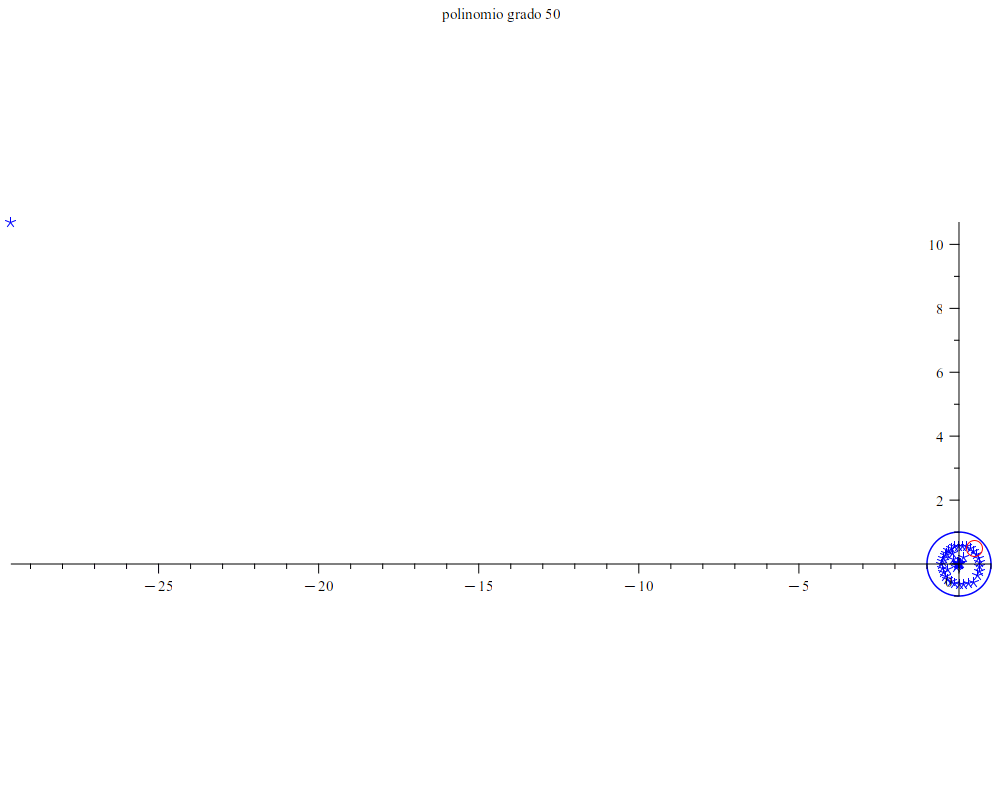
\includegraphics[width=\textwidth]{include/r1_1c1_0c2_(0.5)(0.5)_zeros.png}
	\end{minipage}
\end{center}

\begin{enumerate}
	\item $\lim_{n \to 50}\sigma_{1,n}=\infty$
	\item $\lim_{n \to 50} \rho(\mathcal{D}_{n})=1.999$
	\item $\max\{Z_{n}\}_{n=0}^{50}=2.482$
	\item $\lim_{n \to 50}\sigma_{2,n}=1.498$
\end{enumerate}

\textbf{Ejemplo 8.} % Originalmente Ejemplo 7
$\langle p(z),q(z) \rangle=\int_{S_{0}(1)} p(z)\overline{q(z)}\, dm_{0;1} + p'(0.5)\overline{q'(0.5)}$

\begin{center}
	\begin{minipage}{0.48\textwidth}
		\centering
		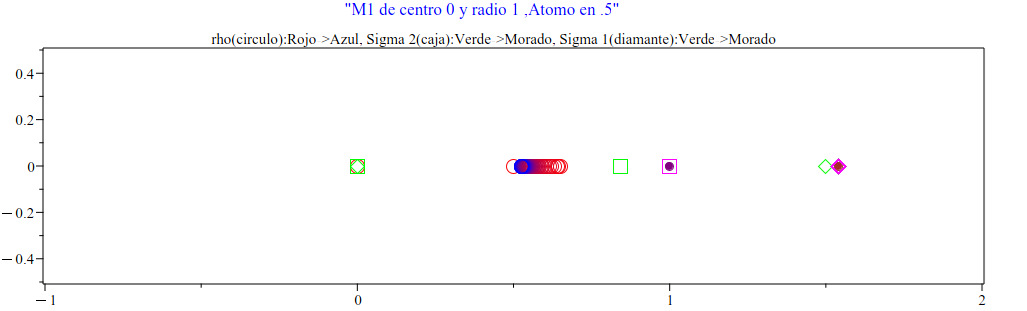
\includegraphics[width=\textwidth]{include/r1_1c1_0c2_0.5.png}
	\end{minipage}%
	\hfill
	\begin{minipage}{0.48\textwidth}
		\centering
		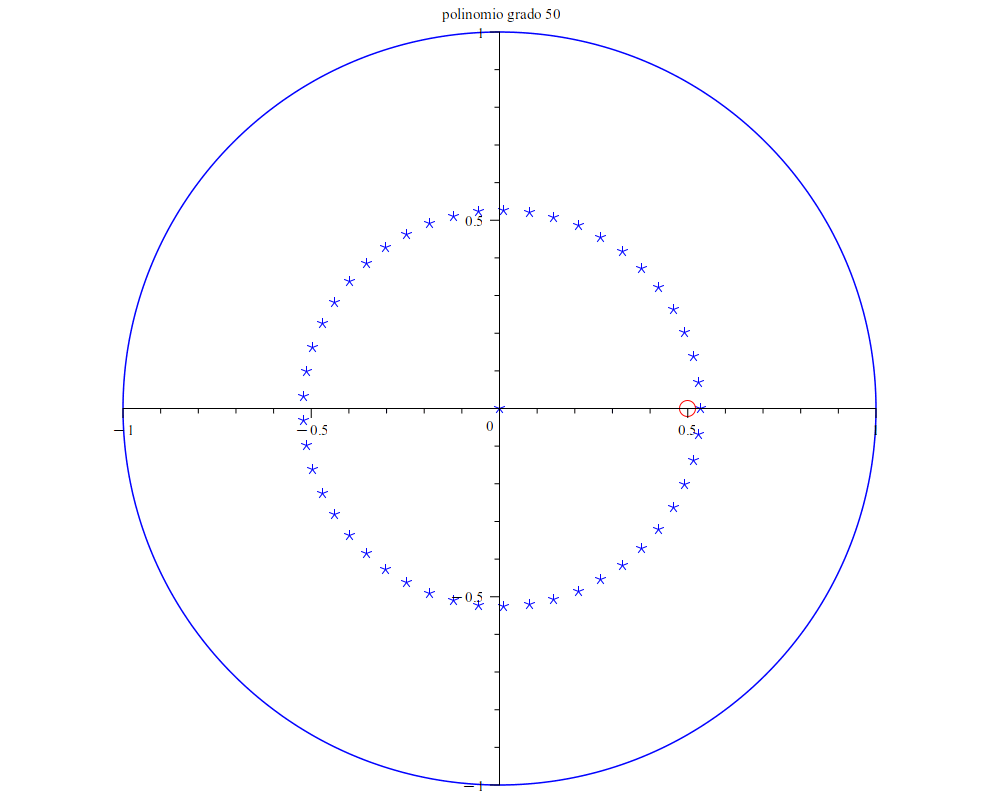
\includegraphics[width=\textwidth]{include/r1_1c1_0c2_0.5_zeros.png}
	\end{minipage}
\end{center}

\begin{enumerate}
	\item $\lim_{n \to 50}\sigma_{1,n}=\infty$
	\item $\lim_{n \to 50} \rho(\mathcal{D}_{n})=2.002$
	\item $\max\{Z_{n}\}_{n=0}^{50}=2.863$
	\item $\lim_{n \to 50}\sigma_{2,n}=0.999$
\end{enumerate}

\textbf{Ejemplo 9.} % Originalmente Ejemplo 8
$\langle p(z),q(z) \rangle=\int_{S_{0}(1)} p(z)\overline{q(z)}\, dm_{0;1} + p'(0)\overline{q'(0)}$

\begin{center}
	\begin{minipage}{0.48\textwidth}
		\centering
		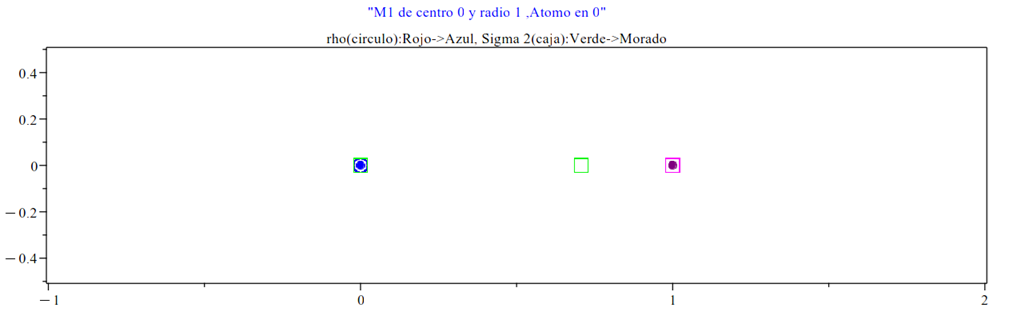
\includegraphics[width=\textwidth]{include/r1_1c1_0c2_0.png}
	\end{minipage}%
	\hfill
	\begin{minipage}{0.48\textwidth}
		\centering
		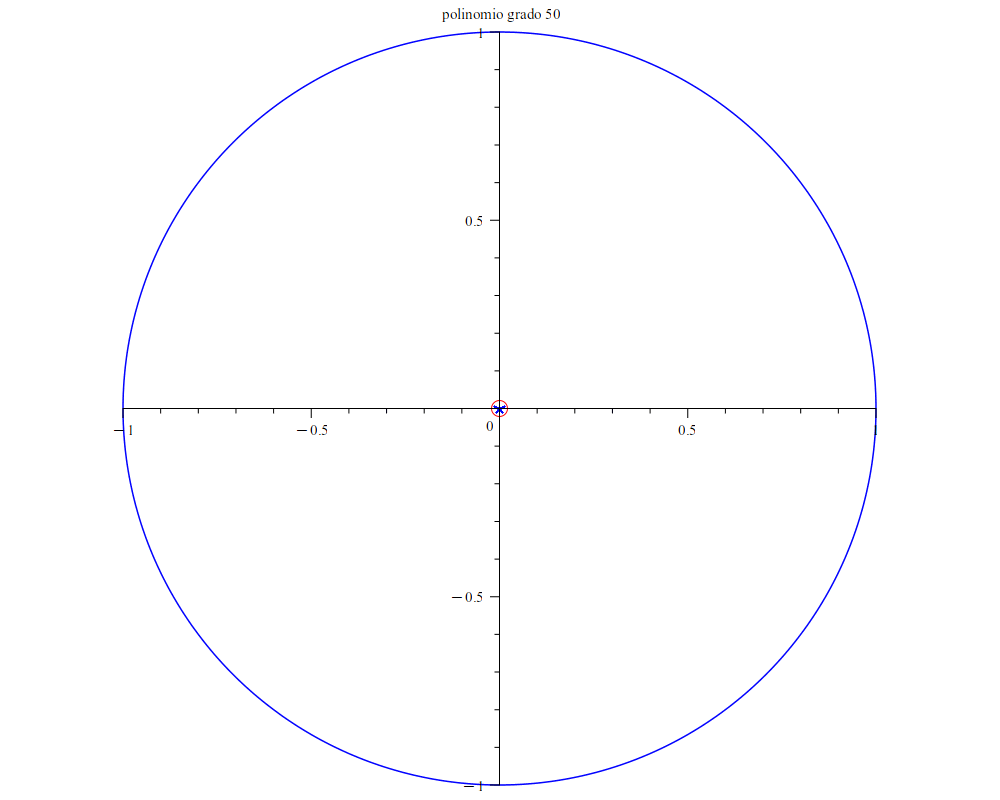
\includegraphics[width=\textwidth]{include/r1_1c1_0c2_0_zeros.png}
	\end{minipage}
\end{center}

\begin{enumerate}
	\item $\lim_{n \to 50}\sigma_{1,n}=\infty$
	\item $\lim_{n \to 50} \rho(\mathcal{D}_{n})=2.000$
	\item $\max\{Z_{n}\}_{n=0}^{50}=2.481$
	\item $\lim_{n \to 50}\sigma_{2,n}=2.000$
\end{enumerate}

\textbf{Ejemplo 10.} % Originalmente Ejemplo 9
$\langle p(z),q(z) \rangle=\int_{S_{0}(1)} p(z)\overline{q(z)}\, dm_{0;1} + p'(0.5i)\overline{q'(0.5i)}$

\begin{center}
	\begin{minipage}{0.48\textwidth}
		\centering
		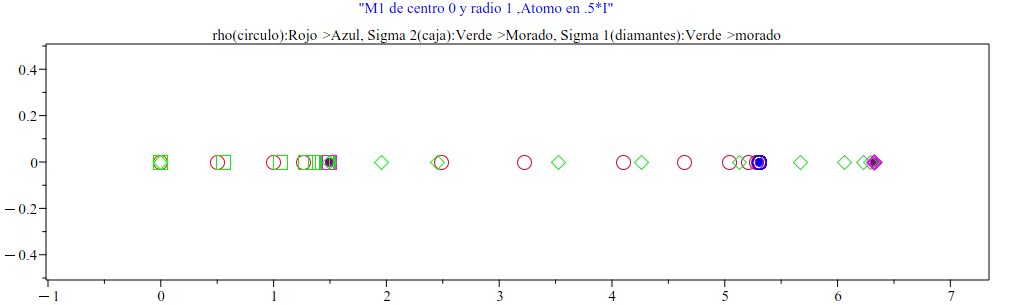
\includegraphics[width=\textwidth]{include/r1_1c1_0c2_(0)(0.5).png}
	\end{minipage}%
	\hfill
	\begin{minipage}{0.48\textwidth}
		\centering
		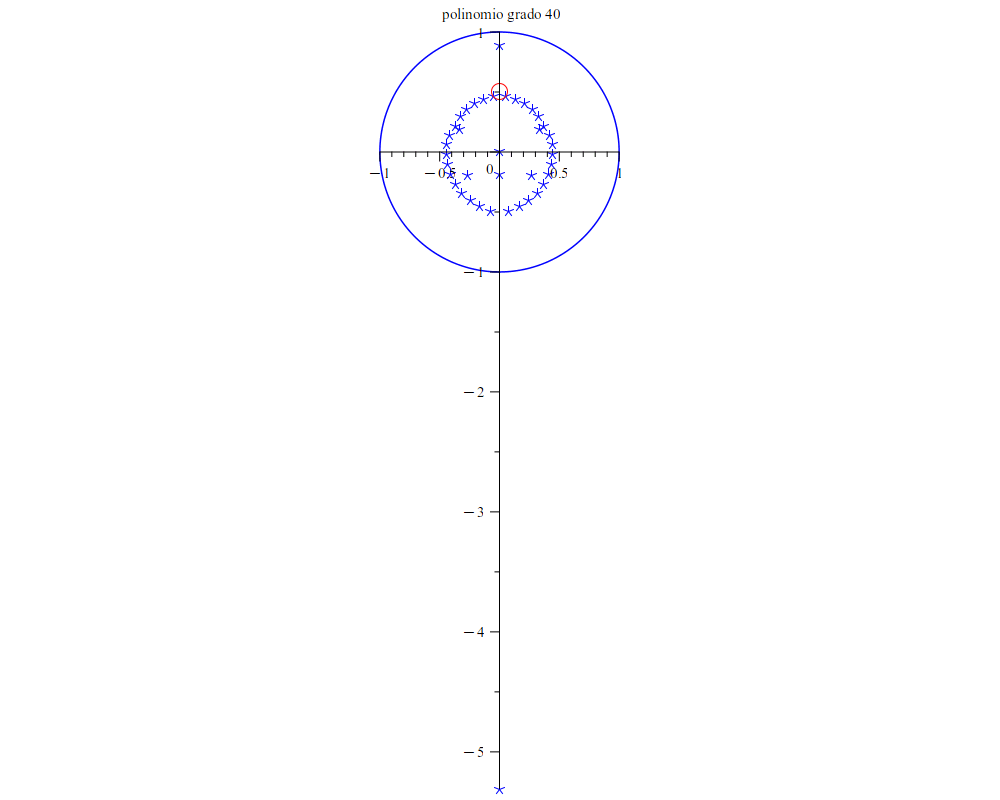
\includegraphics[width=\textwidth]{include/r1_1c1_0c2_(0)(0.5)_zeros.png}
	\end{minipage}
\end{center}

\begin{enumerate}
	\item $\lim_{n \to 50}\sigma_{1,n}=\infty$
	\item $\lim_{n \to 50} \rho(\mathcal{D}_{n})=1.499$
	\item $\max\{Z_{n}\}_{n=0}^{50}=2.257$
	\item $\lim_{n \to 50}\sigma_{2,n}=0.999$
\end{enumerate}

Tras el análisis de los resultados obtenidos en los experimentos con circunferencias, podemos observar patrones similares a los encontrados en el caso real:

\begin{itemize}
	\item Cuando la medida para el producto escalar está soportada en dos circunferencias disjuntas, el radio espectral de $\mathcal{D}_n$ converge al centro más alejado del origen más el radio de su circunferencia.
	\item El segundo mayor valor singular de $\mathcal{D}_n$ parece converger al valor del centro más alejado del origen.
	\item En el caso de productos con átomo, cuando el átomo está fuera de la circunferencia que soporta la medida, los ceros tienden a acumularse cerca del átomo.
	\item Cuando el átomo está dentro o sobre la circunferencia, los ceros se mantienen más próximos a la circunferencia.
\end{itemize}

Estos resultados refuerzan las conjeturas desarrolladas en el caso real y muestran que el comportamiento de los ceros de polinomios ortogonales de Sobolev sigue patrones predecibles tanto en el caso real como en el complejo.

\begin{sidewaystable}
	\centering
	\small
	\caption{Resumen de ejemplos sobre la localización de ceros en el caso de circunferencias.}
	\begin{tabular}{|c|cccc|cccc|cccc|}
		\hline
		\multirow{3}{*}{\textbf{Parámetros}}     & \multicolumn{4}{c|}{\textbf{SECUENCIALMENTE}} & \multicolumn{4}{c|}{\textbf{NO SECUENCIALMENTE}} & \multicolumn{4}{c|}{\textbf{ÁTOMO}}                                                                                                                                                                \\
		                                         & \multicolumn{4}{c|}{\textbf{DOMINADO}}        & \multicolumn{4}{c|}{\textbf{DOMINADO}}           & \multicolumn{4}{c|}{}                                                                                                                                                                              \\
		\cline{2-13}
		                                         & $\sigma_{1,n}$                                & $\rho(\mathcal{D}_{n})$                          & $\max Z$                            & $\sigma_{2,n}$ & $\sigma_{1,n}$ & $\rho(\mathcal{D}_{n})$ & $\max Z$ & $\sigma_{2,n}$ & $\sigma_{1,n}$ & $\rho(\mathcal{D}_{n})$ & $\max Z$ & $\sigma_{2,n}$ \\
		\hline
		\textbf{Ej.1}: $S_{0}(1), S_{0.4}(0.4)$  & $\infty$                                      & 1.000                                            & 1.172                               & 0.998          & -              & -                       & -        & -              & -              & -                       & -        & -              \\
		\textbf{Ej.2}: $S_{0}(1), S_{0.5}(10)$   & $\infty$                                      & 2.632                                            & 3.148                               & 1.997          & -              & -                       & -        & -              & -              & -                       & -        & -              \\
		\textbf{Ej.3}: $S_{0}(1), S_{1}(1)$      & -                                             & -                                                & -                                   & -              & 2.192          & 0.999                   & 1.285    & 0.998          & -              & -                       & -        & -              \\
		\textbf{Ej.4}: $S_{0}(1), S_{-10}(1)$    & -                                             & -                                                & -                                   & -              & $\infty$       & 2.498                   & 2.499    & 2.497          & -              & -                       & -        & -              \\
		\textbf{Ej.5}: $S_{-10}(0.25), S_{0}(1)$ & -                                             & -                                                & -                                   & -              & $\infty$       & 1.998                   & 1.999    & 1.997          & -              & -                       & -        & -              \\
		\textbf{Ej.6}: $S_{0}(1), S_{-10}(0.25)$ & -                                             & -                                                & -                                   & -              & $\infty$       & 2.498                   & 2.499    & 2.497          & -              & -                       & -        & -              \\
		\textbf{Ej.7}: $S_{0}(1), c=0.5+0.5i$    & -                                             & -                                                & -                                   & -              & -              & -                       & -        & -              & $\infty$       & 1.999                   & 2.482    & 1.498          \\
		\textbf{Ej.8}: $S_{0}(1), c=0.5$         & -                                             & -                                                & -                                   & -              & -              & -                       & -        & -              & $\infty$       & 2.002                   & 2.863    & 0.999          \\
		\textbf{Ej.9}: $S_{0}(1), c=0$           & -                                             & -                                                & -                                   & -              & -              & -                       & -        & -              & $\infty$       & 2.000                   & 2.481    & 2.000          \\
		\textbf{Ej.10}: $S_{0}(1), c=0.5i$       & -                                             & -                                                & -                                   & -              & -              & -                       & -        & -              & $\infty$       & 1.499                   & 2.257    & 0.999          \\
		\hline
	\end{tabular}
\end{sidewaystable}